

\title{\papertitle}

\author{Can Paul Bineytioglu,
		Joe Boden,
		Rocco Schulz,\\
		Max V\"{o}kler
		Robert Wawrzyniak}
		
\publishers{Corporate State University\\Baden-Wuerttemberg - Stuttgart}

\date{\today}

\begin{document}
% roman numerals
\renewcommand{\thepage}{\Roman{page}}

%----------------------------------------------------------------------------
% Title Page
%----------------------------------------------------------------------------


\maketitle
% no page numbering on title page
\thispagestyle{empty}

\begin{abstract}
\textbf{\abstractname}: This paper evaluates asynchronous server technologies
using the more recent frameworks Node.js and Vert.x as references. Strenghts and
weaknesses of asynchronous programming models are elaborated to identify areas
where these technologies should be chosen over the common programming
frameworks.
A proof of concept based on Node.js and Vert.x is used to evaluate
non-functional attributes such as maintainability and integration into an
existing application landscape.
\end{abstract}
\newpage






%----------------------------------------------------------------------------
% Table of Contents
%----------------------------------------------------------------------------
\tableofcontents
\newpage


%----------------------------------------------------------------------------
% Abbreviations
%----------------------------------------------------------------------------
% List needs to be indexed after each change.
% This is done by executing the following command:
% ~$ makeindex [filename].nlo -s nomencl.ist -o [filename].nls
\printnomenclature
\addcontentsline{toc}{section}{List of Abbreviations}
\newpage


%----------------------------------------------------------------------------
% List Of Tables
%----------------------------------------------------------------------------
\listoftables
\addcontentsline{toc}{section}{\listtablename}
\newpage


%----------------------------------------------------------------------------
% List of Figures
%----------------------------------------------------------------------------
\listoffigures
\addcontentsline{toc}{section}{\listfigurename}
\newpage

%----------------------------------------------------------------------------
% List of Listings
%----------------------------------------------------------------------------
\lstlistoflistings
\addcontentsline{toc}{section}{List of Listings}
\newpage

% Arabic numerals for page numbering
\renewcommand{\thepage}{\arabic{page}}

% Set page number to 1: 
\setcounter{page}{1} 

\renewcommand{\baselinestretch}{1.4}\normalsize

\section{Introduction}

In traditional web application development data is transmitted synchronously,
i.e. upon a GET/POST request the result can be displayed only after transmission
and processing are finished, as highlighted in figure
\ref{img_req_res}\footcite{req_res}. While maintaining simplicity and
predictability this can cause serious latency when uploading large pieces of
data most commonly complex forms for registration. Naturally rich content such
as images and videos causes even more waiting.

\begin{figure}[hbtp]
\centering
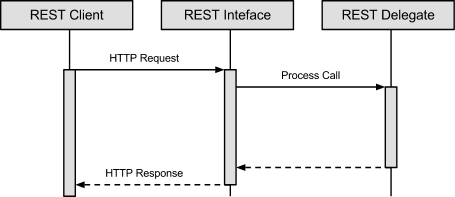
\includegraphics[scale=0.75]{img/rest_call.png}
\caption{REST request-response sequence diagram\label{img_req_res}}
\end{figure}

As demands around collaborative access and media richness evolved, this became a
serious bottleneck, essentially preventing these types of applications. On the
client-, i.e. browser-, side developers were able to work around the issue of
synchronous transmission using the XmlHttpRequest object which allows to request
resources programmatically (using JS\nomenclature{JS}{JavaScript}) while
deferring handling of the response to a callback (see figure
\ref{img_ajax}\footcite{img_ajax}) thus enabling much more responsive software.

\begin{figure}[hbtp]
\centering
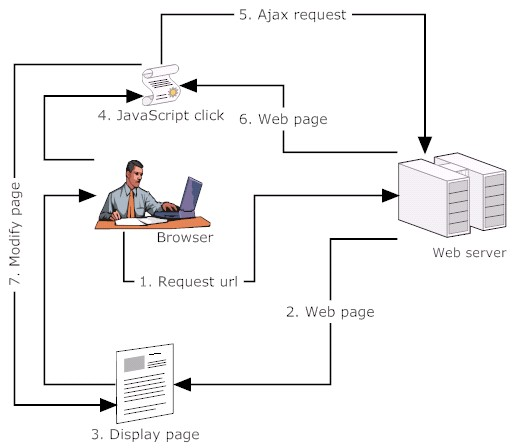
\includegraphics[scale=0.5]{img/ajax-diagram}
\caption{AJAX Diagram\label{img_ajax}}
\end{figure}

Although this addressed the issue on the client-side, server-side request were
still handled very much in a synchronous fashion. For example the popular Apache
web server forks a new process for each incoming request\footnote{TODO: find
source}. As popular applications have to cope with unprecedented amounts of
concurrent users in conjunctions with massive request counts, this obviously
causes performance issues.\\

Relatively young frameworks such as Node.js and Vert.x try to address this issue 
by providing a completely asynchronous programming model which allows associating
multiple simultanious connections with a single thread by using an event-driven approach.

%Goal of this paper and structure
This paper elaborates the concepts behind these young frameworks and analyses their 
technical strengths and weaknesses. Furthermore non-functional attributes will be
evaluated based on two sample implementations in Node.js  and Vert.x.



\newpage
\section{Setting the context}
\label{setting_the_context}

\subsection{Comparison between Asynchronous and Synchronous Processing}
\label{comparison}

%Synchronous calls -> idling threads -> 
A common case in programming is access to I/O.
In synchronous processing a running thread needs to wait for the completion of
the I/O operation before it can continue.
The thread is in an idle state while it is waiting which allows another process 
or thread to occupy the CPU in the meanwhile.\\

% writing multithreaded code is not trivial
In multithreaded applications several threads can run simultaniously within one 
process. Several threads can access shared memory concurrently which can
cause inconcistent states. This can be avoided by synchronizing threads - e.g.
with locks. This means that programmers need to take into account every possible
execution order to effectively avoid program defects such as data races and 
deadlocks.\footcite[Cf.][10]{Breshears_2009}
This can be time consuming and potentially results in error-prone code.

A typical synchronous call is provided in listing \ref{lst:synchronous_call}. The
contents of a file are read and displayed afterwards. The programm is blocked until the
read operation has finished.

% reading a file and displaying it, pseudo code
\lstinputlisting[language=JavaScript,caption={Pseudocode: Synchronously reading and displaying a file's contents},
label=lst:synchronous_call]{lst/synchronous_call.txt}


Asynchronous programming style uses a different concept. The flow of an
application is determined by events, which is why this style is also called
event-driven programming.\footcite[Cf.][16]{teixeira_2012} In listing \ref{lst:asynchronous_call} the call
to the \textit{readAsText} function is done asynchronously. There is no
return value - instead an event handler is provided as a second argument.
This function is also referred to as a callback function. It is called
as soon as the read operation has completed.

% same example as above but with callbacks / events
\lstinputlisting[language=JavaScript,caption={Pseudocode: Asynchronously reading and displaying a file's contents},
label=lst:asynchronous_call]{lst/asynchronous_call.txt}

This concept is coupled with an event loop, which is a single thread that is
running inside the main process.
The loop constantly checks for new events. When an event is detected, the loop
invokes the corresponding callback function. The callback is processed in the
same thread which means that there is at most one callback running at a time.
The event loop continues when the callback has completed. As a result the
developer does not need to take care of concurrency issues during development.
But the developer's task is to write light event handlers that can be processed
quickly as every callback is an interruption of the event processing in the
event loop. \footcite[Cf.][]{Croucher_2010} Memory or processor intense callbacks
can lead to growing queues of unserved events which eventuelly results
in a slow application or service\footcite[Cf.][48]{teixeira_2012}.


% implication: 
% all code should be as non-blocking and asynchronous as possible
% using blocking APIs inside the asynchronous code can cause blocking of the event loop
% which is evil. This is why node.js is based on javacript. Other languages already have
% lots of modules with blocking APIs which could confuse dumb developers.



\subsection{Existing Asynchronous Frameworks}
\label{existing_frameworks}
This sub-section will introduce two upcoming frameworks for server-side asynchronous development: Node.js and Vert.x followed by a brief outline of their potential market success.

\subsubsection{Node.js}
\label{node.js}

To put it in a nutshell one can say, that Node.js is JavaScript on a server.\\
Besides, Node.js is a young platform with a lot of buzz around it. Due to the
rising of the Web 2.0 and widely accessible internet through smartphones,
demanding users expect more complex and more interactive forms of application usage. 
The challenge even gets harder considering the steep number of
devices that are interacting with online services.%TODO: reference?
To overcome those problems Node.js lays it's foundations on an event driven
computing architecture for web servers.\\
% The paradigm of the event driven programming style is easily explained using a
% real world example. What would you do if you are slicing onions while the turkey
% is nearly on fire in the stove? Right, finishing the slice, turning down the
% heat and opening the oven before getting back to slice some onion rings would be
% a reasonable behavior. The truth is, that browser based programming isn't that
% real life oriented. A lot of techniques try to make real-time and parallelism
% work. Which means continuing slicing during you try to safe the turkey.
Node.js doesn't try to make you perform undoable things. It rather lets events drive the
action, so that it is single-threaded and only one thing happens at once. This
is why an event loop is a fundamental part of Node.js. It includes the concept
of nonblocking I/O activities. A result is that actions that cause the program
to wait like database requests and file I/O  do not halt execution until they
return data. In contrast they process independently and raise an event when the
data is accessible. It is therefore necessary to use callbacks for dealing with
different kinds of I/O.\\
An exemplary code for a basic HTTP server in Node.js is shown in listing
\ref{lst:simple_server} to deepen the understandin gof the event loop and
callback in Node.js.

% reading a file and displaying it
\lstinputlisting[language=JavaScript,caption={The simplest way to programm a server in Node.js},
label=lst:simple_server]{lst/simple_server.txt}



The code uses a factory method to create a new HTTP server and attaches the
argument of the createServer function as a callback to the request event. The
first run of this code is also called setup. When a HTTP request arrives the
anonymous callback function is processed and "Hello World" appears on the
browser.\\
That the basic code above isn't the most sophisticated way to write Node.js code
explains the following thought experiment: Assuming that the Hello World page
would be popular and had a lot of requests from different devices to handle and
in addition the callback processing would take one second, it is obvious that the second
request would already have to wait for one second until it gets served. This is far away 
from the near-real-time requirement Node.js is confronted with.\\
Two programming rules in Node.js can be inferred from the basic server and it's
event loop blocking problem, which is described in section \ref{setting_the_context}.
First, once the setup is in place all actions should be programmed event-driven.
Second, if a workload requires Node.js to process something for a long time,
it should be outsourced to web workers.\footcite[Cf.][]{Croucher_2012}

Node.js large performance benefits are caused through the use of Google's new JavaScript engine V8, that ships naturally
with the web browser Chrome. Due to the fact that V8 compiles JavaScript into
real machine code before executing it, Node.js has an advantage over 
traditional techniques such as executing bytecode or interpreting it. \footnote{See \url{https://developers.google.com/v8/intro}}


\subsubsection{Vert.x}
\label{vert.x}

Vertx is a polyglot that runs on the JVM (Java Virtual Machine). It is hence
possible to scale over available cores without manually forking multiple
servers.\\
The application API is exposed in multiple programming lanugages (see table
\ref{tab:existing_frameworks}).
% Implication: use case, code reuse from different legacy systems written in
% different languages

In Vert.x the smallest available deployment unit is a verticle, which runs
inside an instance. Each instance runs singlethreaded.
Multiple verticles can be run inside one instance as depicted in figure
\ref{fig:vertx_constructs}.
%http://vertx.io/core_manual_java.html scaling tcp servers

\begin{figure}[h]
	\centering
	\setlength\fboxsep{2pt}
	\fbox{
	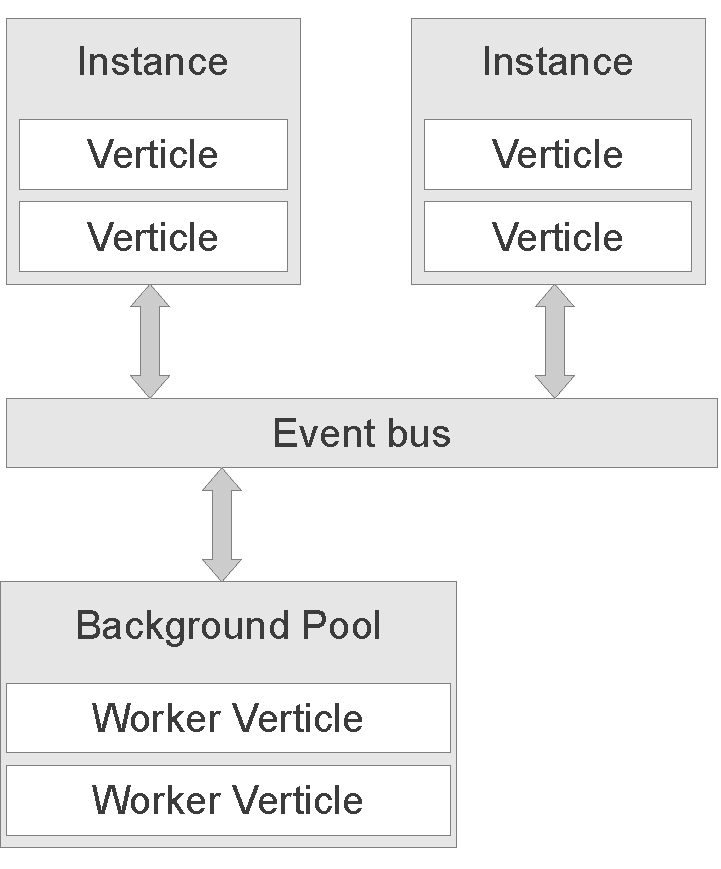
\includegraphics[width=0.4\textwidth]{img/vertx_constructs.pdf}
	}
	\caption{Abstracted deployment units of Vert.x}
	\label{fig:vertx_constructs}
\end{figure}

When multiple instances are run on one machine, Vert.x automatically distributes incoming
requests among all running instances in a round-robin fashion, so that each
vert.x verticle instance remains single threaded.

Vert.x also includes a distributed event bus, which enables verticles to
communicate with each other, either within the same instance or across different
instances. The event bus allows direct communication with in-browser JavaScript as well.\\
% Implication: ideal for real time applications. easy communication between client and server using JS
Vert.x allows to run I/O heavy tasks in separate worker threads that reside in a
so-called background pool as these tasks would otherwise block the event loop as
described in section \ref{comparison}.

The core functionality of Vert.x covers basic networking tasks and protocols,
web servers, clients, access to the file system, shared maps and the event bus.
The core libraries of Vert.x can be embedded in any JVM program for reuse in
larger projects.\\
As opposed to Node.js, the core functionality and API can be considered quite
static as changes need to be done in all supported
languages.\footcite[Cf.][]{vertx_2012}\\ % The core can be extended with
The core can be exctended with additional features that are provided by optional
modules that can be obtained over a public git-based module
repository.\footcite[Cf.][]{vertx_mod_2012}.
The repository currently contains 16 distinct modules in different
versions.\footcite[Cf.][]{Vertx_repository_2012}

%TODO: http://vertx.io/manual.html#message-passing
% add info on message passing. vert.x makes use of shared maps to avoid issues
% in distributed systems. how does node handle that?

An extensive online documentation is available for all supported languages.
Additionally, code examples for most features are available for all supported languages in
a public repository\footcite[Cf.][]{Fox_2013}.\\
Vert.x is open source and licensed under the Apache Software License
2.0\footnote{See \url{http://www.apache.org/licenses/LICENSE-2.0.html}}, so that
commecial redistribution in closed source projects should not be an issue.

\subsubsection{Market Overview}
\label{frameworks_overview}

Table \ref{tab:existing_frameworks} shows that the previously introduced frameworks face stiff competition from established communities (namely the Ruby and Python ones). An important aspect in determining the potential success of a new technology is measuring the interest of software developers in the newcomer. Google-developed Google Trends visualizes the 'search interest', i.e.\ the amount of queries of a particular subject and related ones\footcite{g_trends}.
% TODO insert charts from CSVs found in doc folder

Looking at the charts it can be concluded that interest in Vert.x is low at the moment in absolute terms as well as in relative terms when comparing it to the Node at the same point in its lifecycle.

The gap in interest could be related to many reasons, two of which will be discussed briefly thus concluding this sub-section.

Theory (1) would be that by the time Vert.x became complete enough to develop productively (at least as productive as was possible with Node at the same point), Node already established itself as the dominant technology especially if mindshare is concerned, which is supported by the data from Google.
Theory (2) is based around technical considerations. Because of the dogmatic nature of asynchronicity in the Node.js framework, every package available on NPM\nomenclature{NPM}{Node Package Manager} is built with asynchronous calling and non-blocking I/O\nomenclature{I/O}{Input / Output} in mind. Vert.x on the other hand is in a curious position here, Vert.x itself is architecturally similar to Node but its ecosystem of established Java libraries is not developed with these principles in mind. This poses the danger of executing synchronous/blocking code, negating all of Vert.x' advantages. Obviously this can limit interest from the outset.

\FloatBarrier

\begin{savenotes} %alloows proper citation marks inside tables
\begin{longtable}[c]{p{0.2\textwidth} p{0.15\textwidth} p{0.57\textwidth}}
\toprule
\textbf{Name} & \textbf{Language/s} & \textbf{Description} \\
\midrule 
\endhead
Twisted			& Python			& ``Twisted is an event-driven networking engine written in 
									  Python and licensed under the open source MIT license"\footcite[Cf.][]{Twisted_2012}.
									  Twisted is a mature framework with a large number of supported networking
									  protocols. Its development is backed by an active
									  community.\footcite[Cf.][12]{fettig_2005}
									  \\
									  
EventMachine 	& Ruby    			& ``EventMachine is a library for Ruby, C++, and Java
									  programs. It provides event-driven I/O using the Reactor 
									  pattern."\footcite[][]{eventmachine_2012}\\

Node.js			& JavaScript		& Node is based on Chrome's JavaScript runtime \textit{V8}.
									  The platform is fully event-driven and offers core
									  functionalities for network programming. Its functionality
									  can be extended with a large number of modules using an
									  integrated package management system.
									  Node.js started development in 2009 and the community
									  is growing since that.\footcite[Cf.][]{Mashtable_2011}\\
									  
Vert.x			& JavaScript, Java, Python, Groovy, Ruby, Coffeescript		
									& A JVM based platform for network applications which is
									  inspired by Node.js. Vert.x comes with its own event
									  bus system that allows distributing applications
									  among multiple network nodes. Support for the languages
									  Scala and Clojure is scheduled for future releases.\footcite[Cf.][]{vertx_2012}\\
\bottomrule 
  \caption{Existing asynchronous programming frameworks}
  \label{tab:existing_frameworks}
\end{longtable}
\end{savenotes}


\FloatBarrier


\newpage
\section{Areas of Application}
\label{areas_of_application}

\subsection{Use Cases}
\label{use_cases}
The non-blocking nature of asynchronous calls is important in all types of
applications that need to handle a large number of requests in real time.\\
Some success stories are available on \url{http://nodejs.org/}.

Could be used for: 
\begin{itemize}
  \item networked applications that tend to keep many inactive connections
  \item web trackers
  \item web servers
  \item lightweight json APIs (non-blocking I/O model 
  		combined with JavaScript make it a great choice for
  		wrapping other data sources such as databases or web 
  		services and exposing them via a JSON interface)%see http://nodeguide.com/convincing_the_boss.htm
  \item proxies
  \item email and messaging systems
  \item authorization processors
  \item Streaming data (e.g. file uploads in real time)
\end{itemize}

\subsection{Don't use cases}
\label{dont_use_cases}


As with all technologies one has to carefully evaluate whether or not it suits the
requirements of a project. Besides those use cases listed in the previous
section there are also a few usage scenarios where one should not use
asynchronous frameworks like Node.js or Vert.x.\\
In general it can be said that these frameworks are not suited for tasks that
require a lot of computation and IO access. These heavy tasks would have to be
moved to worker threads. However having most of the computation logic in
constructs that are not of the event loop contradicts the point of these
frameworks. Running worker threads does partially introduce concurrency issues that were
avoided with the event loop again as multiple threads could concurrently access IO.\\
Another thing to note is that one should not choose these frameworks when
there are other concepts or frameworks that might better fulfill the 
projects requirements.
A selection of such cases is shown in the list below. 

Criticism on these concepts:\\
\url{http://xquerywebappdev.wordpress.com/2011/11/18/node-js-is-good-for-solving-problems-i-dont-have/}\\
\url{http://www.theserverside.com/discussions/thread.tss?thread_id=61693}\\
\url{http://static.usenix.org/events/hotos03/tech/full_papers/vonbehren/vonbehren_html/index.html}\\
and some more. Why not use message queues that make use of a thread pool?

Node.js and Vert.x do not offer any possibility to speed up a single request. These requests will aways
run at the same speed. What it does is to maximise the number of possible requests while keeping the speed
steady. This is why it scales so well. The only additional delay between request and response is the time
that a request waits in the event loop until it gets processed.\\
In many cases however it is desirable to minimize the computation time itself for a single request.
Once this is achieved it becomes a goal to keep that speed for a larger amount of requests.

\begin{description}
  \item[Datawarehousing with analytics] Doing analytical and complex computations
  	on large data sets at runtime usually requires a lot of computing power.
  	It can be expected that each request will require quite some time to be processed.
  	This computation time cannot be shortened much when run on a single thread but 
  	could potentially be speed up significantly when run on multiple cores in parallel. 
  \item[CRUD / HTML applications] \nomenclature{CRUD}{Create Read Update Delete}
	This refers to classical websites that basically only serve as an interface for
	an object relational model.
	At present Node.js and Vert.x do not provide additional benefits to scalability
	for these types of web applications. Unless the page has to deal with a large number of
	concurrent requests it should be considered to use a more powerfull frameworks
	like Ruby On Rails, Grails or Django. These are currently better suited for quickly
	developing such an application. Providing a site that is suited for 
	millions of requests does not automatically increase the number of users.
\end{description}
    

    


\newpage
\section{Exemplary Implementations}
\label{exemplary_implementations}

A simple web form application has been implemented in Node.js and Vert.x to
further analyze non-functional requirements and collect practical experience
with these frameworks. These implementations are thoroughly described in the following sub-sections.

\subsection{Software Description}
\label{software_description}
\FloatBarrier
The exemplary implementation consists of a web service that can be used to calculate
the expected fee for an insurance. However this application should only serve as a 
demonstration of the used asynchronous frameworks and is hence very simplified.

\begin{figure}[h]
	\centering
	\setlength\fboxsep{2pt}
	\fbox{
	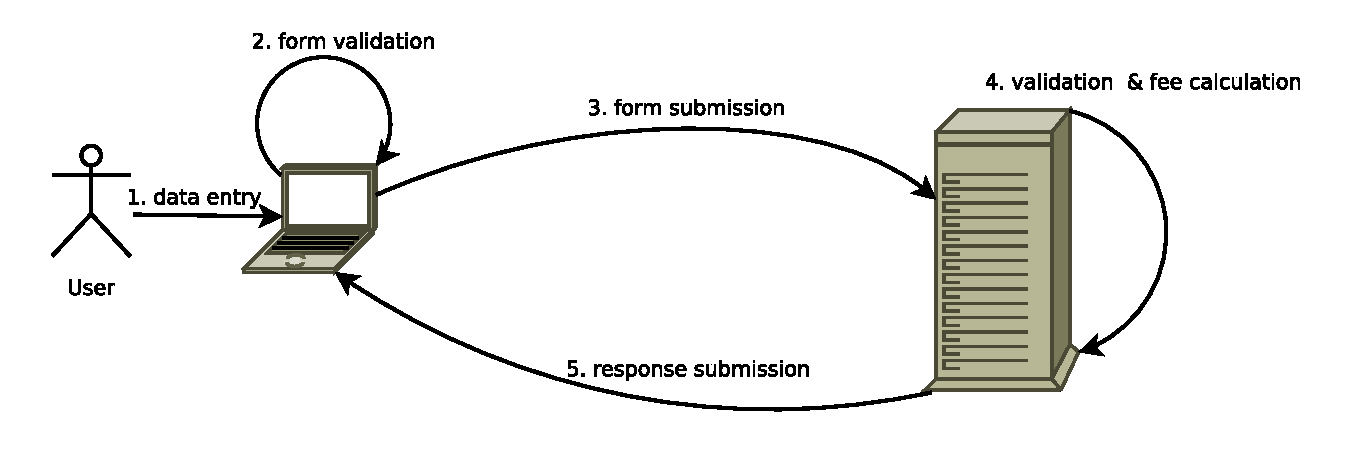
\includegraphics[width=0.9\textwidth]{img/poc_workflow.pdf}
	}
	\caption{Usage workflow of the exemplary application}
	\label{fig:application_workflow}
\end{figure}


The basic usage workflow is shown in figure \ref{fig:application_workflow}. In a
first step the user opens the website in a browser and is shown a form that
consists of two parts - the first part being a section for personal details and
the second part for parameters that will be used to determine the fee for the
insurance.\\
The user then fills in all necessary form fields and instantly gets feedback on
the vailidy of the entered values. Once all fields are filled correctly the form
can be submitted to the application via HTTP or HTTPS. The data received by the server
then gets validated again to avoid processing of manipulated requests. Eventually
the valid data is passed into the calculation routine which returns its result
to the user by triggering the according callback.

\nomenclature{HTTPS}{Hyper Text Transfer Protocol Secure}
\nomenclature{HTTP}{Hyper Text Transfer Protocol}





\FloatBarrier
\subsection{Software Design}
\label{software_design}

\nomenclature{CSS}{Cascading Style Sheets}
\nomenclature{HTML}{HyperText Markup Language}

This simple usage scenario leads to a few requirements and
design decisions.
The user interface has to consist of HTML, CSS and JavaScript files as it 
will be displayed in a web browser. In general these files are not initially
available on the clients machine and need to be delivered via HTTP by the
server. These file requests are usually done via GET.\\

\begin{figure}[h]
	\centering
	\setlength\fboxsep{2pt}
	\fbox{
	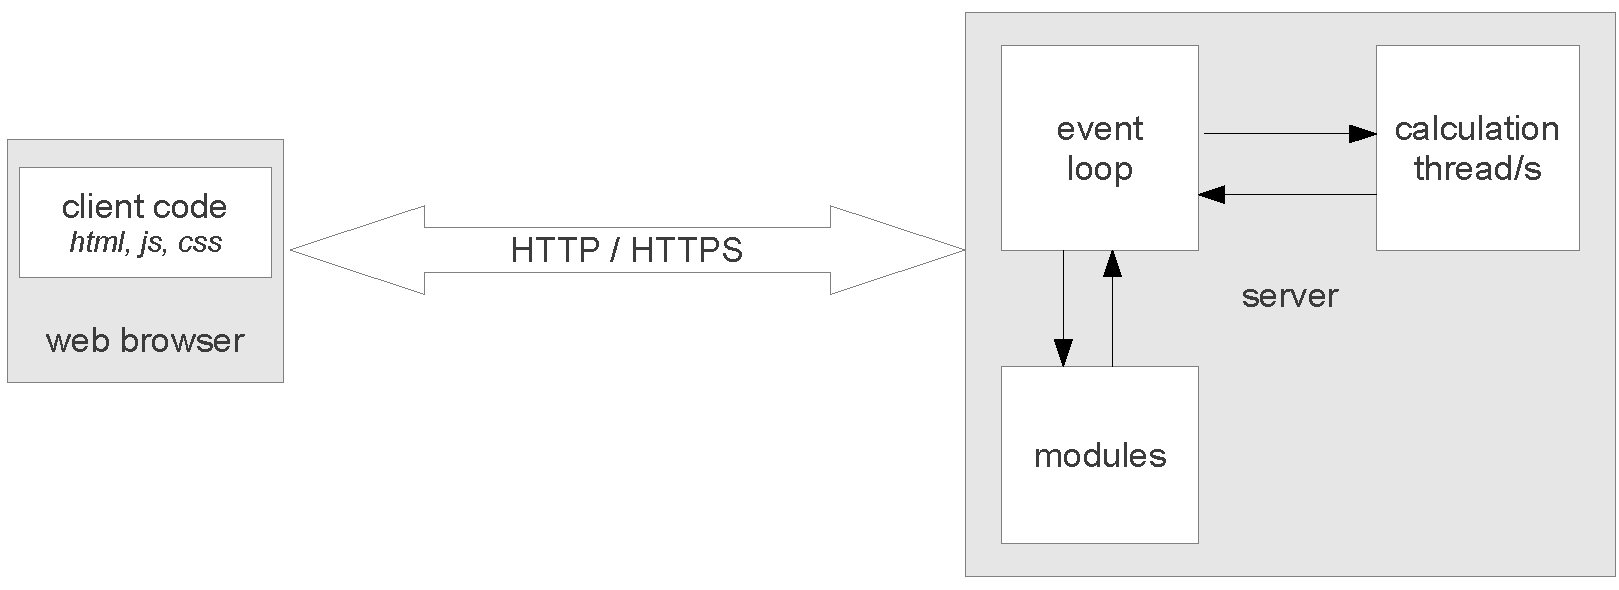
\includegraphics[width=0.8\textwidth]{img/high_level_architecture.pdf}
	}
	\caption{High level architecture of the application}
	\label{fig:application_workflow}
\end{figure}

In addition to the static files, the server will also need to process
requests that are sent via POST in order to receive the form data for the
fee calculation.\\
The body size of these requests is fairly small as the submitted values consist
of plain text only. Therefore it is safe to assume that it won't be necessary to
buffer each part of the requests body but start calculating once the data
submission has completed.\\
In reality these calculations are much complexer than in this simple scenario,
so that they have to be done outside of the event loop in a separate thread.
In the implementation these long running calculations are simulated artificially for
demonstration purposes.\\
Additional features in the backend can be integrated via existing modules from
the repositories of Vert.x or Node.js.



\FloatBarrier
\subsection{Software Implementation}
\label{software_implementation}

\subsubsection{Vert.x}
\label{implementation_vertx}

The vertx application is written in Java entirely, but it is also possible to
write each verticle in a different language if desired. This could be done to
maximize code reuse between frontend and backend.\\
The business logic of the backend consists of three verticles and additional
utility classes.
One verticle serves as a web server that accepts HTTP and HTTPS requests. GET
requests are interpreted as file requests and are answered directly from within
the verticle. POST requests are interpreted as form submissions. Whenever a POST
requests arrives the verticle transforms the request body to a Json object and
submits it via Vert.x' event bus.\\
The second verticle is a worker verticle which does the CPU intense calculation
tasks.This verticle listens on the event bus for incoming messages. Whenever
such a message arrives it transforms the received Json object into a form
instance for validation and fee calculation.The results are then sent back via
the event bus of this operation has completed, so that the event loop can return
the result to the client in its next iteration.\\
The third verticle serves as a starter script which programmatically starts
the previously mentioned verticles and terminates afterwards as it does not
define any callbacks itself (see listing \ref{lst:starter_verticle}).

\lstinputlisting[language=Java,caption={Verticle that starts two other verticles},
label=lst:starter_verticle]{lst/starter_verticle.java}

The actual deployment of the other verticles happen in lines 13 and 14.
An important detail is the 2nd parameter in the \texttt{deployWorkerVerticle} method.
Vert.x allows deploying multiple instances of a verticle programmatically
which eases scaling an application to the number of available processors of a machine.
In this case the main loop is single-threaded and for each remaining processor
there is one worker verticle. Vert.x automatically distributes requests among
these worker verticles (as described in section \ref{vert.x}).

A global configuration file is read in line 12. These configuration file is
formatted as Json string and can include settings for modules or verticles. The
path to the configuration file has to be provided to the \texttt{vertx} command
upon server start to allow access to it from within the verticles. For this implementation the command that
has to be invoked is shown in listing \ref{lst:vertx_start}.

\lstinputlisting[language=bash,caption={Command for starting the Vert.x application},
label=lst:vertx_start]{lst/vertx_start_command.sh}

Vert.x allows either running verticles by providing the compiled Java class or by providing the
source file which is then compiled automatically by Vert.x. However in this
setup we experienced some issues with the Vert.x run command when we tried to
use it with the source files. The issues observed where partially related to
Vert.x bug 444\footnote{see \url{https://github.com/vert-x/vert.x/issues/444}}.
Due to incomplete dependency resolution, not all classes were compiled so that
Vert.x could not find all required classes in the path at runtime.
These startup issues can easily be avoided by using compiled classes instead of
the source files when multiple verticles need to be started programmatically.
The path to the compiled classes has to be provided with the \texttt{cp} switch as
shown in listing \ref{lst:vertx_start}.


\lstinputlisting[language=Java,caption={Command for starting the Vert.x application},
label=lst:vertx_form_handler]{lst/vertx_form_handler.java}


The implementation of the communication between the web server and the worker
verticle was rather easy by using the event bus. The event bus has a very
simple adressing mechanism where the address consists of a normal string.
Listing \ref{lst:vertx_form_handler} shows the form handler which is defined
in the web server verticle and gets called whenever a form submission arrives.
The handler registers another handler that is called as soon as the entire
request body has arrived (line 3). The data that arrives as a buffer is than
turned into a JsonArray (line 7) and submitted to the event bus (line 9).
As soon as a reply is returned over the event bus it is forwarded to the client (line 12).



\subsubsection{Node.js}
\label{implementation_node}
The node.js implementation starts with four modules that are required to run the application:


% reading a file and displaying it
\lstinputlisting[language=JavaScript,caption={HTTP and HTTPS in Node.js},
label=lst:simple_server]{lst/http_https.txt}


The HTTP and HTTPS modules are necessary to set up the webservers accordingly. 
In addition, the “fs” (FileSystem ) module is necessary to read the encryption keys for HTTPS.
 The web framework “Express” offers complementary functionality for a webserver, like routing, 
and will therefore be used for convenience purposes, as recommended by Roden, G. (2012). 
Express can be installed using the following command-line command:

npm install express 

To demonstrate an HTTP and HTTPS server likewise, the application includes two webservers, 
both of which serve the same functionality. In order to enable HTTPS by leveraging 
the node.js class https.Server, it is necessary to generate a pair consisting of a private 
and a public key, because the handshake prior to an HTTPS session follows a specific procedure :
 (1) Client contacts the server using a secured URL.
 (2) The server responds sending the digital certificate to the browser.
 (3) The client certifies that the certificate is valid (e.g. by trusted authorities).
 (4) Once the certificate is validated, the one-time session key generated by the client will be used to encrypt all communication with the server.
 (6) The client encrypts the session key with the public key of the server. Only the server can decipher the data using the private key.
The generation of private and public keys can be done be using the following commands, leveraging OpenSSL, an Open Source toolkit to implementing secure protocols :

\begin{lstlisting}[caption={Generating a new pair of public/private keys}]
openssl genrsa -out privatekey.pem 1024
openssl req -new -key privatekey.pem -out certrequest.csr 
openssl x509 -req -in certrequest.csr -signkey privatekey.pem -out certificate.pem
\end{lstlisting}
As soon as the privatekey.pem and certificate.pem files are available, their content can be written into the httpsOptions array by using the FileSystem module and its function readFileSync():

% reading a file and displaying it
\lstinputlisting[language=JavaScript,caption={FileSystem module},
label=lst:simple_server]{lst/filesystem.txt}


The files in this example are located in the same location as the application file. To run the HTTP/HTTPS servers, the following code is used:

% reading a file and displaying it
\lstinputlisting[language=JavaScript,caption={Running the server},
label=lst:simple_server]{lst/serverrun.txt}



The HTTP server can be accessed using http://localhost:8888/ as opposed to the HTTPS server that is available at https://localhost:4431/.

To be able to use Express, a variable called “app” will be initialized:

% reading a file and displaying it
\lstinputlisting[language=JavaScript,caption={App variable},
label=lst:simple_server]{lst/appVariable.txt}



The first Express functionality used is that static files can be served with node.js. Using the following statement, the directory “/UI” is made the root directory for a http://localhost:[port]/
\begin{lstlisting}[language=javascript,caption={Serving static assets with Express}]
app.use(express.static(__dirname + '/UI'));
\end{lstlisting}
Another Express feature is the “bodyParser”, which is used as middleware to parse request bodies, for this Proof of Concept especially JSON.

\begin{lstlisting}[language=javascript,caption={Using the $bodyParser$}]
app.configure(function(){
    app.use(express.bodyParser());
});
\end{lstlisting}

Moreover, Express is used to catch requests to specific URLs. As the AJAX call coming from the user interface is set up as POST-request, the following code shows how to catch this (AJAX-driven) POST-request in node.js on http://localhost:8888/insurances:

\begin{lstlisting}[language=javascript,caption={Handling an HTTP POST request with Node.js}]
app.post('/insurances', function (req, res) {

// iterating through the array that contains JSON-objects
// write the value of the “name” attribute of each JSON-object into the console
    for(var i = 0; i < req.body.length; i++) {
        console.log(req.body[i].name);
}

    res.contentType("text/plain");
res.send(200, OK)

}
\end{lstlisting}

As the AJAX POST-request contains an array filled with JSON-objects, this example demonstrates how to access each item. Within the proof of concept, this for-loop is used to apply regular expressions in order to validate each form field.

The node.js servers can be started by using the command-line. After navigating into the project’s folder using cd, the only command needed is:
\begin{lstlisting}[caption={Executing Node.js code}]
node [filename].js
\end{lstlisting}


\newpage
\section{Evaluation of Non-functional Attributes}
\label{evaluation_nonfunctional}

\subsection{Maintainability}
\label{maintainability}
Maintainability is one of the most important issues in the enterprise for developers typically switch between projects (or participate only in a temporary manner). Thus the time needed to become familiar with a framework and its language directly impact the development cost either because of the time needed related to the learning curve or because of resources invested in maintenance and bug-fixing.
The results of this sub-section are summarized in table \ref{tbl_maintain}.\\

\paragraph{Node.JS}
Node.js allows for leveraging the JS skills already in the market which significantly lowers the Time to Market (TTM\nomenclature{TTM}{Time to Market}) for its similarity to established libraries and conventions in web application development. Unfortunately TTM is not everything because equal attention needs to be given to Total Cost of Ownership (TCO\nomenclature{TCO}{Total Cost of Ownership}), i.e.\ the total expenditure required including costs incurred post-deployment. Here Node presents a challenge in its reliance on callback leading to hard-to-follow and hard-to-fix code driving up TCO significantly because patches become more and more difficult to write with increasing $\Delta t_{Launch<->Present}$, especially if the code is not to be maintained by the original developers.

Furthermore, Node is still at an unstable stage of code maturity (at time of writing, the current version is $0.9.6$ causing infrequent breaking changes to its APIs which usually is a no-go in the enterprise, this is reinforced by a community mindset of 'Upgrade Node, Update Code' based on a preference for new features. The unintended benefit of this is a lot of available material for Node programmers in blogs and on StackOverflow\footnote{\url{www.stackoverflow.com}} leading to the conclusion that the current pace of progress does not facilitate enterprise adoption, however it is not a showstopper.

\paragraph{Vert.x}
Vert.x offers a similar picture to Node, however some of Node's shortcoming are more pronounced on the Vert.x side of things. Whereas Node can recruit from established web developers, is Vert.x suffering from a curious conundrum. It is based on the JVM, which has enormous amounts of talent (esp. in the enterprise) but because of its diametrical differences to the conventional libraries it does not seem to be able to recruit interest from this pool. Also its support for multiple programming languages (basically every JVM language) should lower the barrier for entry even more, as for example Groovy already features Vert.x-aligned language constructs. Unfortunately this means that new Vert.x programmers need to be trained increasing TTM significantly.
Another important issue is the unstable state of the Vert.x codebase as essential features like code import do not work reliably or at all\footnote{TODO: INCLUDE REF TO BUG}. Section \ref{frameworks_overview} already mentioned the ease of calling synchronous code with Vert.x though this can be worked around with by placing the code in new verticles, this still requires a lot of vigilance.

TCO is difficult to estimate for Vert.x for a lack of success/failure stories, it can be said though that because Vert.x requires Java hosting infrastructure ther emight be an associated licensing cost for application servers.

\begin{table}[hbtp]
\centering
\begin{tabular}{|c|p{5cm}|p{5cm}|}
\hline 
• & Node.js & Vert.x \\ 
\hline 
Skill Availability & Good & None \\ 
\hline
Skills Transferable? & Yes (from est. JS frameworks) & No (very different from conventional J2EE\nomenclature{J2EE}{Java 2 Enterprise Edition} \\
\hline
Available Material & A lot (books, blogs, documentation) & Project documentation \\
\hline
License Cost & None & None \\
\hline
TTM & Low (transferable skills + material) & High (learning curve) \\
\hline
TCO & Medium (low TTM but may be high maintenance) & Medium (takes longer to develop, but JVM maintenance is well known) \\
\hline
\end{tabular} 
\caption{Maintainability comparison of Node and Vert.x}
\label{tbl_maintain}
\end{table}

\subsection{Integration}
\label{integration}
Vert.x and Node.js are supposed to be used as fully event driven standalone
applications that can be extended with event-driven modules.
However when introducing a Node.js or Vert.x application into the current
application landscape it might be desired to reuse or communicate with existing
systems that are not fully event driven. Furthermore, integration of these technologies might not be limited to mere IPC\nomenclature{IPC}{InterProcess Communication} but instead as a new middleware-layer beneath current and new applications.\\
%Consider connecting that software with a message bus.
%Separate IO intense tasks into ``web workers'' or similar constructs.

\subsubsection{Node.js Integration}
\label{node_integration}
Node.js is not designed to handle CPU-intensive tasks efficiently. However,
there is a way a Node process can perform such tasks without impairing the
application performance. Node.js uses so-called child processes for this
(provided by the \textit{child process}
module). The module is basically a wrapper around the unix tool \textit{popen} and
provides access to a child process' communication streams (stdin, stdout, stderr).
\footcite[Cf.][]{node_child_process}

There are two cases child processes are used for:\\
First, CPU-intensive tasks can be performed outside Node by assigning them to a
different process (which is then called a child process) in order not to block
the event loop. Output data from the child process is then sent back to the
parent process.\footcite[Cf.][63]{teixeira_2012} In this case, the child process is used to
outsource a task that requires high computation work and would otherwise block
the event loop. This approach however requires routines that should run
within the child process to be written in JavaScript as well, so that it is not
usable to properly connect an existing application with the Node application.\\
A second way of using the child process module is to actually run external
commands, scripts, files and other utilities that cannot directly be executed inside Node.\footcite[Cf.][63]{teixeira_2012}

This characteristic lets external processes get well integrated with Node.js.
A basic example of the child process module is shown in listing \ref{lst:node_child}\footcite[Taken from][]{node_child_process}.
The child process instance that is created in lines 1 and 2 is an event emitter that
allows registering callbacks for certain events (see lines 4,8 and 12).

\lstinputlisting[language=JavaScript,caption={Example of running \textit{ls -lh /usr} in Node.js, capturing stdout, stderr, and the exit code},label=lst:node_child]%
{lst/node_child_process.js}


Invoking processes on a different machine across the network still
requires a remote API or a distributed message bus system.


\subsubsection{Vert.x Integration}
\label{vertx_integration}
In Vert.x there are multiple ways to communicate with external programs.
Depending on the used language there are already multiple libraries that can be
used to invoke child processes. However these libraries usually only expose
synchronous APIs, so that these calls need to be done inside a worker verticle
that doesn't block the event loop.\\

Listing \ref{lst:vertx_child} shows a minimal worker verticle written in
Java that invokes \textit{ls -lh /usr} via the \textit{Apache Commons Exec}
library.\footnote{See \url{http://commons.apache.org/exec/}}

\lstinputlisting[language=Java,caption={Example of running \textit{ls -lh /usr} in Vert.x from within a worker verticle},label=lst:vertx_child]%
{lst/vertx_child_process.java}

When writing verticles in Java it is also possible to make use of Javas Remote
Method Invocation (RMI) mechanism to communicate with services that are on different
machines in the network.
The most natural way for inter-application communication is by either using the
integrated message bus or by using a separate bus system.
Vert.x can be embedded in any JVM based program by including the according
libraries in the path, so that these applications can use the bus system as
well.\footcite[Cf.][]{vertx_2012}

\subsubsection{Middleware}
\label{middleware}
Middleware is a layer of software providing standardized access to resources for many consumers and to increase code reuse. The JVM\nomenclature{JVM}{Java Virtual Machine} and its associated libraries building the foundation for Vert.x are a classic example of this concept. The following sub-sub-section uses mostly examples from the Node.js community although they are also valid for Vert.x.

The underlying concepts of both frameworks outlined thus far in this paper present advantages to middleware/library development as it does for business logic implementation. This realization manifests itself not only in the number of packages available on $npm$ (TODO: INSERT NUMBER + REF HERE) but also in new projects built on top of Node.

\paragraph{Meteor and Opa}
Meteor and Opa are two frameworks built on top of Node.js and MongoDB created around a radically new development workflow. Both eliminate the distinction between client-side and server-side code, instead the developer writes code in a very similar way to conventional desktop programming. The difference (and main selling point) is that the framework decides at runtime (TODO: VERIFY WITH DOCS) which piece of is executed on the server or transmitted to the client for execution. An example of this methodology can be found in appendix \ref{appendix1}.

The interesting part of these new frameworks beside the obvious is that by utilizing Node every part of the stack immediately becomes asynchronous and non-blocking. By further abstraction away from 'bare-metal' Node, leveraging its inherent advantages becomes much easier including enhanced code maintainability (TODO: VERIFY).

\paragraph{Etherpad}
Etherpad is an online collaborative text editor. Etherpad nicely illustrates the power of Node as middleware. By migrating to Node reductions of lines of code and memory usage(TODO: REF FROM GITHUB) allow for easier embedding in web applications and also greater extensibility by offering a JS API\nomenclature{API}{Application Programming Interface}.


% TODO insert image


\subsection{Scalability}
\label{scalability}
Support for single machine scaling using multiple threads exists.
Deployment on distributed systems differs in node.js and vert.x.
Vert.x. uses its own communication bus to share information between verticles.
Vert.x uses Hazelcast's\footnote{See \url{http://www.hazelcast.com/}} clustering functionality internally to scale on multiple machines. 


\section{Conclusion}
\label{conclusion}

%----------------------------------------------------------------------------
% APPENDIX
%----------------------------------------------------------------------------
% Appendix sections need to be within the subappendices environment.
% Use the command \appsection{title} instead of \section to introduce each
% appendix. This will add each appendix to the list of appendices.

% sets the appendix environment and resets the section counters
\newpage \begin{appendices} 
\appendixtocon %adds an 'Appendices' entry to the toc

\appendixpage %prints the title on the page

\subsection*{\listappendixname}
%--------------------------------
% style of the \listofappendices command is defined in header.tex
\listofappendices

% begin appendices on a new page
\newpage

%start environment for subappendices, so that new sections are formatted as
%subsections of appendix
\begin{subappendices}
\renewcommand{\setthesubsection}{\arabic{subsection}:}%


\appsection{METEOR OR OPA EXAMPLE}
% include your appendix with the LaTeX include command
\label{appendix1}
CODE CODE CODE

%--------------------------------
% close the appendices environment
\end{subappendices}
\end{appendices}